% position image in center
\begin{figure}[h]
    \centering
    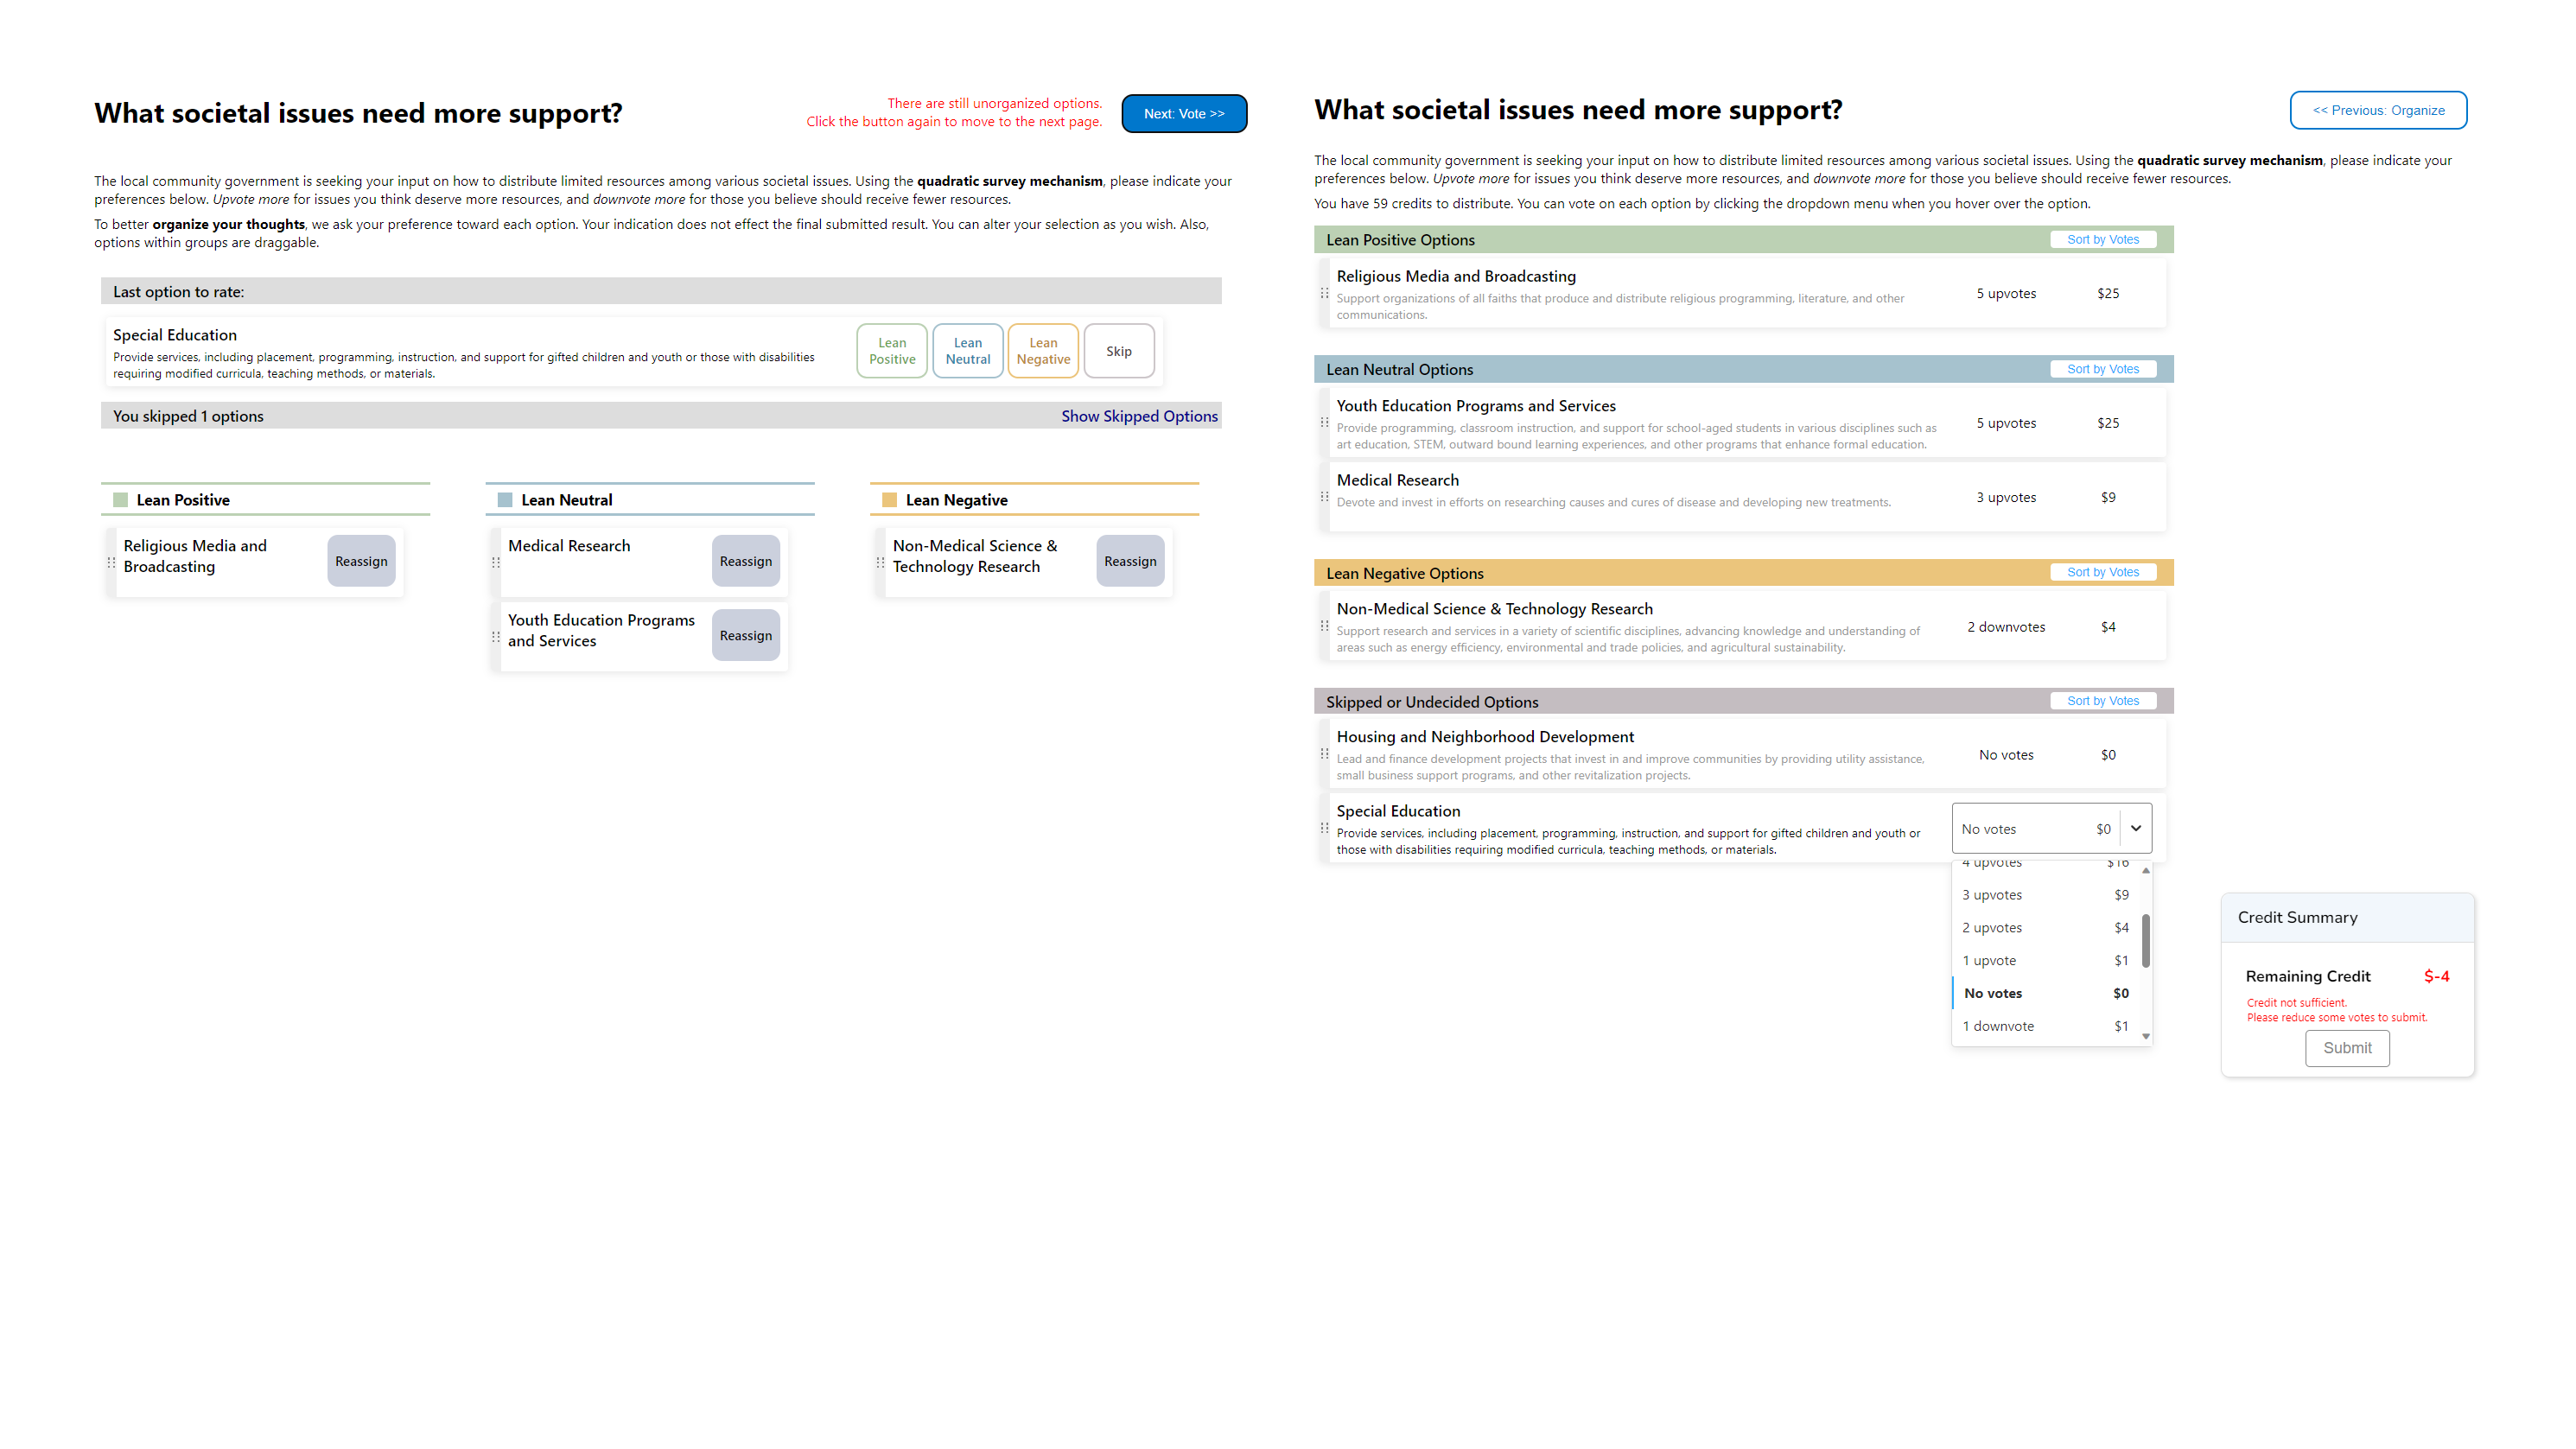
\includegraphics[width=1\textwidth]{content/image/interface.png}
    \caption{The interactive interface}
    \label{fig:interactiveInterface}
\end{figure}

\section{Experiment Design}
To answer our research questions, we developed an open-source system with an interface specifically for quadratic surveys. We then designed a two-by-two mixed-method experiment to examine how the number of options and the interface type affect the participants. This section details each experiment component.

\subsection{System Design}
We designed an interactive text interface (ITI) and a baseline text interface (BTI) for this study. We begin from describing BTI. In order to better understand the influence of number of options and different interface components to support QS, we identified essential components for QS (detailed deliberation in appendix.). Unlike many prior studies, we intentionally removed all data visualization elements as inappropriate visualizations might increase mental demand [Huang, Measuring Effectiveness of Graphs, 2009] rather than reduce the demand. Thus, in the BTI interface (Figure X), participants are presented with a list of options with a system prompt on top. Each option has a dropdown that provides all possible voting options and cost given the number of credits. A small summary box is to the right of the interface showing the current cost and the remaining credit.

The ITI interface (Figure Y) builds on top of the BTI interface with two additional components. The first acts as a scaffolding process to support an opportunity for individuals to first organize their thoughts before they vote. The interface would show individuals all options presented in the QS one at a time. Respondents can choose to place the option into one of the three ordinal categories -- lean positive, lean negative, or lean neutral. Respondents can also choose not to and move on to the voting page if they wish. In other words, we designed an interface to nudge survey respondents to review and group different options. As the survey respondent decides to move on, the interface seamlessly transitions to the voting page where options' positions reflect how they were organized and displayed, including the order within each category. These orders were preserved unless the survey respondents directly manipulate its position. The second component of the BTI interface allows participants to drag-and-drop options anytime during the voting process, whether it is during them organizing the options, or when respondents are voting, individuals can readjust the position of the options, to convey agency to the interface. Participants are aware that these additional interface interaction designs will not influence the voting outcome.

These designs are informed from prior literature. The purpose of the information organization is to design a simple, straightforward mechanism to create positional proximity such that options with similar preferences are positioned close by. This design is informed by the proximity compatibility principle \cite{wickens1995proximity}, specifically spatial proximity~\cite{wickens1990proximity}, and mental compatibility. In other words, the interface should present information that is processed together and the mental model of how the task is completed in order to reduce cognitive load. The notion of drag-and-drop has been explored widely in rank-based surveys. For instance, \textcite{krosnick2018measurement} demonstrated that replacing drag-and-drop with traditional number-filling rank-based questions improved participants' satisfaction with a little trade-off in their time. A similar work embedded drag-and-drop as part of its ranking process \cite{timbrook2013comparison}. Even though drag-and-drop interface might lower the stability of the outcome, since we are not trying to capture the position of the options as our final solution, it is worth its trade-off for which survey respondents express a higher satisfactory affordability and ease of use~\cite{rintoulVisualAnimatedResponse}.

We hypothesize that showing one option at a time forces survey respondents to focus on expressing their preferences independently, without introducing the cognitive load that comes from the ranking process. The interface uses these high-level information to inform the relative positions that dynamically present how the options were placed on the layout. Due to the proximity of related options, survey respondents would be able to expend less cognitive effort when expressing their ratings using the QV mechanism. In addition, the interactive interface allows survey respondents to interpret, organize, and make fine-grained adjustments with real-time feedback to align with design principles, affordances, agency, feedback, and constraints outlined in \cite{norman2013design}.

The system is designed using a React.js frontend and a next.js backend powered on MongoDB. Both systems are open-sourced.

\subsection{Study Setup}
We recruited participants from a midwestern college town using online ads, digital bulletins, social media posts, physical flyers, and online newsletters. The study's researcher prioritized the non-student population to maximize participant diversity.

A visual presentation of the study protocol is provided in Figure K. Participants were invited to the lab for the study. This in-lab study was designed for two primary reasons. First, as we measured cognitive load, it was crucial to minimize the influence of external factors that could affect this measurement. Such factors, more prevalent in remote experiments or those conducted via platforms like MTurk, include potential multitasking or interruptions by others. Second, conducting the study on a consistent device enabled control over the participants' interface. A 32-inch vertical monitor was specifically chosen to display the interface, reducing the need for scrolling. Since cognitive load includes the mental effort to process information in working memory, it was important to minimize cognitive load arising from hidden options. The vertical monitor setup allowed for the display of all options simultaneously.

Upon adjusting the screen's angle and height, participants digitally signed a consent form. They then watched a video explaining QS operations, sans interface, followed by a short quiz. Participants could view the video multiple times, if desired. The quiz's purpose was not to screen out participants but to ensure their understanding of QS mechanics. Participants had the opportunity to ask questions after both the video and quiz.

The researcher then guided participants through a QS on societal issues. System design randomly assigned participants to one of four study groups at the start. The groups were as follows:
\begin{itemize}
    \item 6 options with BTI
    \item 6 options with ITI
    \item 24 options with BTI
    \item 24 options with ITI
\end{itemize}
Participants completed the survey independently, without the researcher's presence. Upon completion, they contacted the researcher, who then requested they complete the NASA-TLX to assess cognitive load. This was followed by a short semi-structured interview to gain insights into the participants' experiences. Finally, participants completed the situational motivation scale (SIMS) to gauge motivation, and a demographic survey. The session concluded with a debriefing and a \$15 cash compensation for their participation.

The study is designed as a between-subject study for two reasons. First, we aim to minimize the study fatigue that might occur given the complexity of responding to a QS. We choose not to ask participants to revisit the lab with several days in between, to reduce dropout rates and prevent demotivating participants from attending the in-person experiment, which might occur in a within-subject study design. Second, we aim to reduce the learning effect that is difficult to remove, especially concerning operating the interface and making decisions on the survey. We want to ensure that participants are not influenced by their previous experience when completing the survey.

An ideal setup to understand participants' cognitive load across multiple options would require enumerating all possible numbers of options and eliciting the "breaking point" where the participant experiences cognitive overload. Unfortunately, this is not feasible. Iterating through all possible numbers of options is very costly, both in time and resources. Therefore, we refer to prior literature to inform our choice of 6 and 24 options, representing a short and long list of options. To decide the number for the short list, survey methods such as constant sum surveys and Analytic Hierarchy Process (AHP) recommend options fewer than ten and seven, respectively~\cite{moroneyQuestionnaireDesignHow2019, saatyGroupDecisionMaking2013, saatyPrinciplesAnalyticHierarchy1987}. However, we are not aware of any specific works that justify these numbers. ~\textcite{saatyPrinciplesAnalyticHierarchy1987} associated this value with both the cognitive processing capacity of $7\pm2$ ~\cite{miller1956magical} and a theoretical proof using the consistency ratio of a pairwise comparison metric~\cite{saaty2003magic}. This informs our decision to contain a pair of dependent variables above and below seven options. We turn to experiments designed to study choice overload. A meta-analysis by~\textcite{chernev2015choice} surveyed 99 choice overload experiments (N = 7202) and summarized that 6 and 24 are the modal values for short and long lists when testing choice overload. These two values are likely rooted in the original choice overload experiment by~\textcite{iyengarWhenChoiceDemotivating2000}. The value six is often used in experiments to understand the effect of choice provision. The value 24 is the maximum number of ecologically valid jams produced by the jam company in the original study. We decided to follow suit with these two values, satisfying the previous decision to choose two values less than and greater than seven.

Next, we describe the context of the survey that participants completed. Participants were asked to complete a societal issue survey. We follow suit as described by \textcite{chengCanShowWhat2021}, believing that surveying societal issues is a good topic as it is relevant to every citizen and it is easy to convey that there are limited resources in the public sector to be prioritized across different sectors and areas. Participants across all four groups were presented with options randomly drawn from 26 societal issues. These issues were generated from the categories used by Charity Navigator~\cite{CharityNavigatorAnimals2023}, a non-profit organization that evaluates over 20 thousand charities in the United States. The full list of these societal issues is provided in the appendix.


Last, we describe the two quantitative measurements taken during the study: cognitive load and motivation. At the time of this study, several methods existed to measure cognitive load, including performance measures, psychophysiological measures, subjective measures, and analytical measures~\cite{gaoMentalWorkloadMeasurement2013}. Given the nature of QS, a task requiring a long period, adopting performance measures like secondary-task measures in our experiment proved challenging due to the difficulty of designing a secondary task. The secondary task must use the same cognitive resources as the primary tasks, and the cognitive resource for completing the survey would vary among participants. Similarly, psychophysiological measures such as pupil size~\cite{palinkoEstimatingCognitiveLoad2010} and ECG~\cite{haapalainenPsychophysiologicalMeasuresAssessing2010} can be highly sensitive to external environments and costly to obtain. Consequently, we relied primarily on subjective measures via self-report surveys and analytical measures like time and clicks collected via the interface. We adopted a paper-based weighted NASA Task Load Index (NASA TLX), a multidimensional scoring procedure using the weighted average of six subscale scores to represent overall workload. Weighted NASA-TLX uses a priori workload definitions from subjects to weight and average subscale ratings, requiring subjects to evaluate each weight's contribution to the workload of a specific task~\cite{hart1988development, hartNasaTaskLoadIndex2006a, cain2007review}. This approach reduces between-rater variability, indicating differences in workload definitions among raters within a task and variations in workload sources between tasks~\cite{cain2007review}. Despite criticisms regarding its validity and vulnerability, NASA-TLX is commonly used due to its low cost and ease of administration~\cite{gaoMentalWorkloadMeasurement2013}. It has been tested on various experimental and lab tasks, and workload scores derived from these tests showed significantly less variability among evaluators than one-dimensional workload scores~\cite{rubioEvaluationSubjectiveMental2004}. Thus, we chose NASA-TLX to measure cognitive load in our study.

In addition to NASA-TLX, we administered a situational motivation scale (SIMS) to measure participants' motivation (required citation). We posited that motivation would influence mental demand (required citation). SIMS, chosen for its widespread use, helps understand one's intrinsic motivation, extrinsic motivation, identified regulation, and external regulation, and was originally designed to measure self-determination. Both instruments were administered using pen-and-paper.